\section{CNN from Scratch}
This chapter shows the results of the training of several custom architecture, that have been defined in order to solve the classification task.
Starting from a very simple model, we start to analyze how to improve it and what modifications to apply in order to improve performance, taking into account mainly the accuracy on the validation test, but also considering other metrics like training time or number of parameters.
The overall strategy is the following:
\begin{itemize}
\item test of different custom architectures defined from scratch
\item analysis of the level of fitting, try of different techniques to fight possible underfitting/overfitting
\item Experiment with the addition of Batch Normalization
\item hyperparameters optimization on the best model so far using a Genetic Algorithm(see Section 2.6)
\end{itemize}

The objective of the presented procedure is not the total exploration and exploitation of the search space, but it aims at finding good results in a reasonable time exploiting an ad-hoc heuristic search.
The tested models are the following:

\subsection{Standard CNN}
\subsubsection{Simple model}
The first experiment has been conducted using a customized standard CNN that exploits Convolutional Layers and max Pooling to process input images. To start, we defined a very simple model, whose structure is reported in the image \ref{fig:standardCNN}. This network is mainly a starting point of our trial-and-error approach and will give us a first approximation of what is going to be our prediction power on the considered task.
\begin{figure}[H]
	\centering
	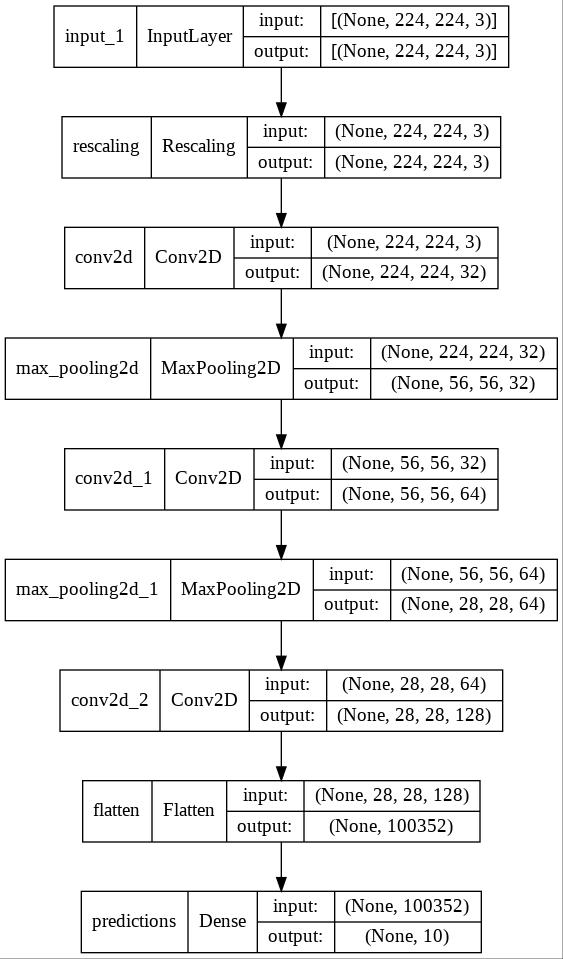
\includegraphics[height=0.6\textwidth]{img/scratch/standardCNN.jpg}
	\caption{Customized Standard CNN Architecture}
	\label{fig:standardCNN}
\end{figure}

\noindent This model is trained using these default hyperparameters:
\begin{itemize}
\item optimizer: \textit{ADAM}
\item dropout rate :0.0
\item learning rate: optimizer's default
\item batch size: 128
\item learning rate decay: none
\end{itemize}

\noindent In particular, we set a large value for batch size both because our main goal is to maximize the accuracy and also (as presented in the Introduction) to face off with the great variability of paintings with very dissimilar style but belonging to the same author. In this way, we increase the probability of a batch to be "complete", thus being representative of this variability.

\noindent The results obtained are the following:

\medskip

\begin{tabular}{ |p{2cm}|p{2cm}|p{2cm}|p{2cm}|p{2cm}|  }
\hline
\multicolumn{5}{|c|}{StandardCNN} \\
\hline
\textbf{Epoch stopped} & \textbf{Validation Accuracy} & \textbf{Testing Accuracy} & \textbf{Validation Loss} & \textbf{Testing Loss} \\
\hline
15 & 0.5730 & 0.786 & 1,3656 & 0.6542\\
\hline
\end{tabular}

\medskip


\begin{figure}[H]
	\begin{subfigure}{0.5\textwidth}
		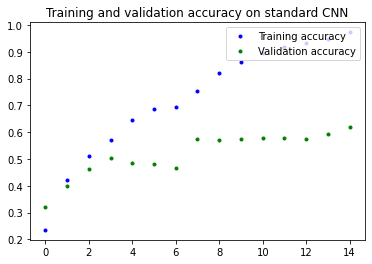
\includegraphics[width=0.9\linewidth]{img/scratch/standardCNN_results_accuracy.png} 
		\caption{Standard CNN Accuracy}
		\label{fig:standardCNNacc}
	\end{subfigure}
	\begin{subfigure}{0.5\textwidth}
		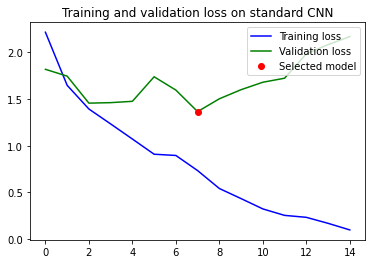
\includegraphics[width=0.9\linewidth]{img/scratch/standardCNN_results_loss.png}
		\caption{Standard CNN Loss}
		\label{fig:standardCNNloss}
	\end{subfigure}
\end{figure}

\medskip

\noindent The network reaches an accuracy value equal to 57.3\% in just 8 epochs, then it overfits very quickly. It can be caused by mainly 3 factors:
\begin{itemize}
\item Data available is insufficient, so the network loses the ability to generalize
\item Lack of regularization techniques, such as Dropout or L1/L2 regularizations
\item \textbf{The spatial extent of the feature map of the last layer is still quite large, so the fully connected layers have too many parameters operating in a quite shallow representation. } 
\end{itemize} 

\subsubsection{Deeper network and dropout}

